\documentclass{beamer}
%\usepackage{pgfpages}
\setbeameroption{show notes on second screen}

\usepackage{hyperref}
\usepackage{xcolor}
%\usepackage[dvipsnames]{xcolor}
\usepackage{tikz}
\usetheme{Luebeck}
\usecolortheme{magpie}

\definecolor{Turquoise}{rgb}{0.0, 1.0, 0.94}

\beamertemplatenavigationsymbolsempty


\title{Unsupervised Deep Embedding for Clustering Analysis}
\subtitle{Bachelorseminar Data Mining}
\author{Lukas Mahr}
\institute{Ludwig-Maximilians-Universität München}
\date{}


\graphicspath{{images/}}
\setbeamertemplate{headline}{}
\begin{document}

\begin{frame}
\titlepage
\end{frame}


\begin{frame}[plain]{Roadmap}
\tableofcontents
\end{frame}

\section{Clustering of high dimensional data}
\begin{frame}[t]{Clustering of high dimensional data}\vspace{4pt}
\begin{itemize}
\item Probleme
%\pause
\begin{itemize}
\item unwichtige Features
%\pause
\item lange Cluster Zeiten
%\pause
\item Komplexität von z.B. KMeans
%\pause
\item $O(n^{dk+1})^{\text{\cite{Kmeans}}}$k=anz. Clusters, n=anz. Elemente, d=Dimension
\end{itemize}
%\pause
\item Idee / Lösungsansatz 
\begin{itemize}
%\pause
\item Feature/Dimension Reduktion
%\pause
\item in Abhängigkeit der Clustere
\end{itemize}
\end{itemize}
\note{viele Daten Punkte viele Distanzen zu berechnen
schwierig zu visualisieren ohne die Dimensionen zu reduzieren
Komplexität von Kmeans die exponentiell ansteigt}
\end{frame}

\section{Einleitung zu Neuronalen Netzen}
\subsection{Idee}
\begin{frame}[t]{Einleitung zu Neuronalen Netzen}\vspace{4pt}
\begin{center}
\begin{itemize}
\large\item[] Nicht-lineare statistische Modelle zur Informationsverarbeitung
\large\item[] Informationsverarbeitung umfasst hierbei unter anderem
\begin{itemize}
\item[] Klassifikation
\item[] Prognosenerstellung
\end{itemize}
\large\item[] Units der Neuronalen Netze angelehnt an Neuronen
\begin{itemize}
\item[] Inputs zusammenfassen
\item[] Mit Schwellenwert vergleichen bzw. aktivieren
\end{itemize}
\large\item[] Verbindungen zwischen Units angelehnt an Synapsen
\begin{itemize}
\item[] Gewichtung mit verstärkender oder schwächender Wirkung
\end{itemize}
\end{itemize}
\end{center}
\note{
wofür braucht man neuronale Netze\\
- Klassifizierung von Daten\\
- Prognose eines bestimmten Wertes\\ 
- Neuronen an Neuronen in unserem Gehirn angelehnt\\
- Verbindungen zwischen Künstlichen Neuronen an Synapsen angelehnt\\
- supervised learning = überwachtes lernen\\
-- man besitzt Daten mit Beschriftungen (labels)\\
- unsperviesed learning nicht überwachtes lernen\\
-- unbeschriftete Daten, also es sind keine labels vorhanden\\
}
\end{frame}

    
\subsection{Künstliches Neuron}
\begin{frame}[t]{Einleitung zu Neuronalen Netzen}\vspace{4pt}
Künstlichen Neurons
\begin{figure}
    \centering
        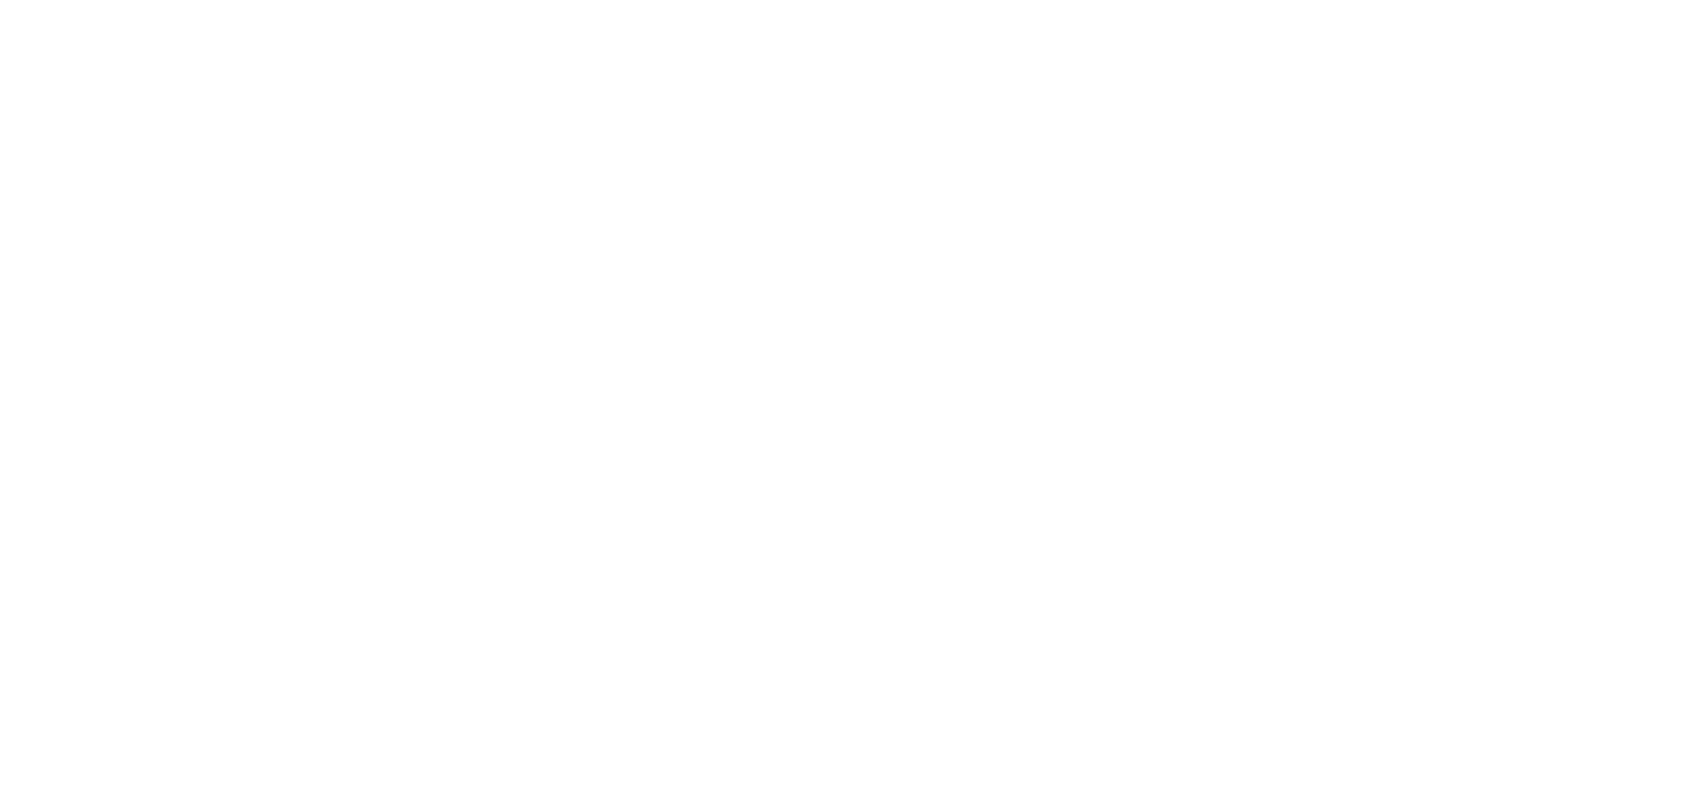
\includegraphics[width=0.8\textwidth]{ArtificialNeuronModel_deutsch_invers.png}
		\tiny\caption{Darstellung eines künstlichen Neurons mit seinen Elementen \tiny\url{https://de.wikipedia.org/wiki/Datei:ArtificialNeuronModel_deutsch.png}}
\end{figure}
\note{
$x_1, ..., x_n$ sind die input variablen, jede der Eingabe variablen besitzt ein
Gewicht, $w_{1j}, ..., w_{nj}$. Diese werden Multipliziert und davon dann die summe berechnet. Hier die Übertragungsfunktion. Dazu wird ein Bias, in dem Fall der Schwellenwert gerechnet. Als letztes gibt es noch die Aktivierungsfunktion die meistens 
einen Wert zwischen 0 und 1 zurückgibt. Das ist dann der input für das nächste Neuron. 
}


\end{frame}

\subsection{Layer/Schicht}
\begin{frame}[t]{Einleitung zu Neuronalen Netzen}\vspace{4pt}
Layer/Schichten
\begin{figure}
    \centering
        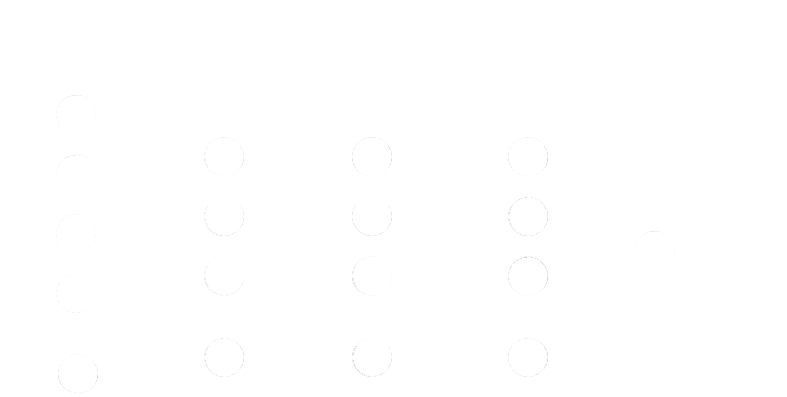
\includegraphics[width=0.8\textwidth]{network-layers-invertiert.png}
		\tiny\caption{Deep learning Künstliches neuronales Netz maschinelles lernen Apache MXNet - mehrschichtige PNG \tiny\url{https://de.cleanpng.com/png-x3zkr7/}}
\end{figure}
\note{Layer/Schicht sind mehrere Neuronen die mit allen Neuronen des nächsten Layer/Schicht verbunden sind. Alle Neuronen in einem Layer haben die gleiche Aktivierungsfunktion. Hidden Layer haben meistens die Aktivierungsfunktion rectified linear, da diese recht einfach und schnell zu berchnen ist. Das outputlayer hat meistens eine etwas kompliziertere Funktion wie softmax oder sigmoid. Abhängig von der Aufgabe des Netzwerkes. Letztes Layer hier direkt mit dem Loss}
\end{frame}

\subsection{Aktivierungsfunktion}
\begin{frame}[t]{Einleitung zu Neuronalen Netzen}\vspace{4pt}
Aktivierungsfunktionen
\begin{figure}
    \centering
        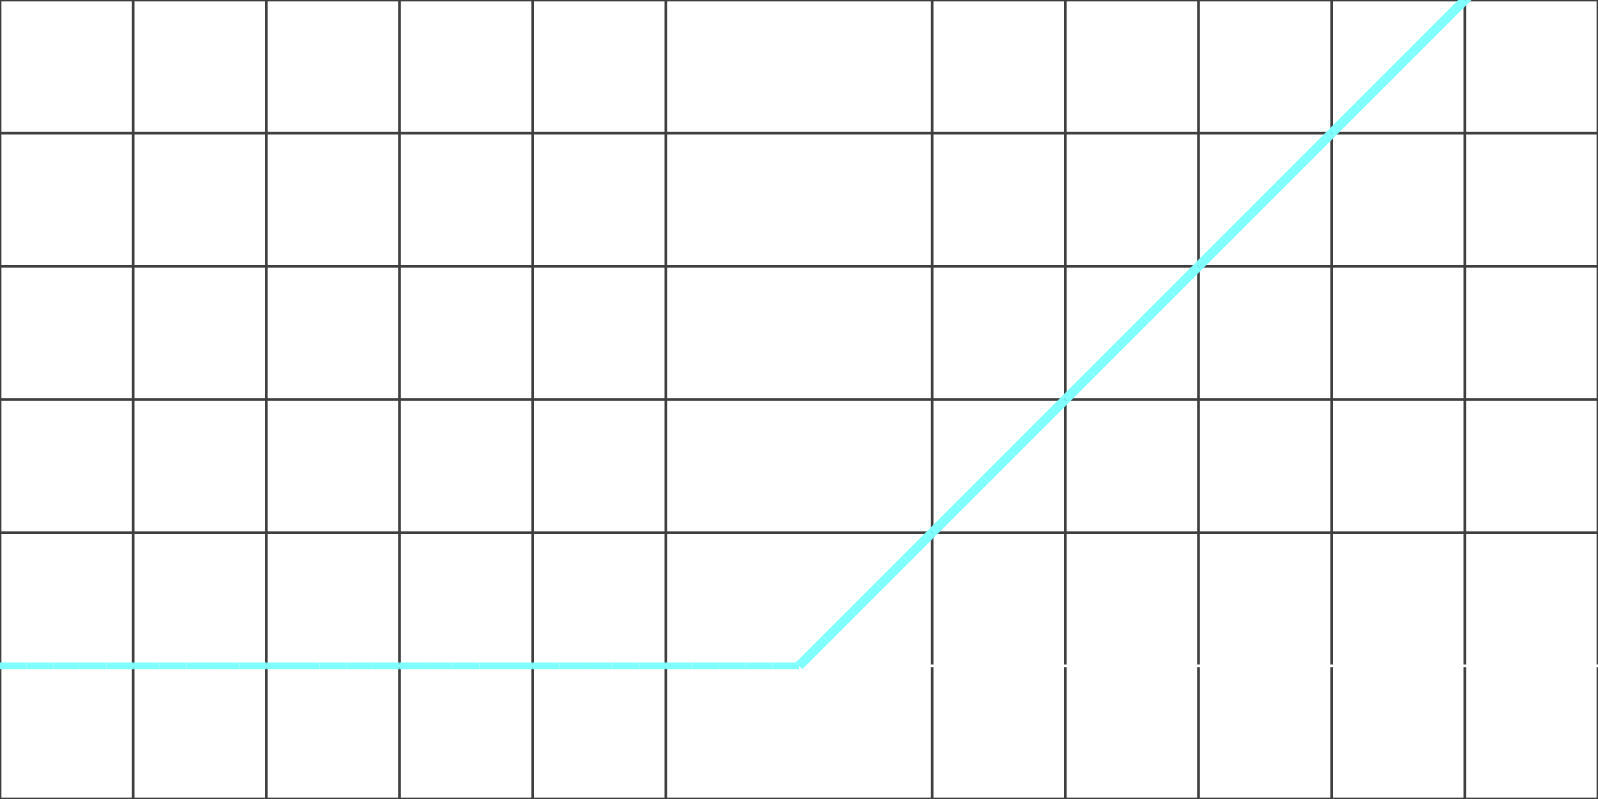
\includegraphics[width=0.4\textwidth]{Activation_rectified_linear_invertiert.png}
		\tiny\caption{Rectifier-Aktivierungsfunktion \tiny\url{https://de.wikipedia.org/wiki/Datei:Activation_rectified_linear.svg}}
		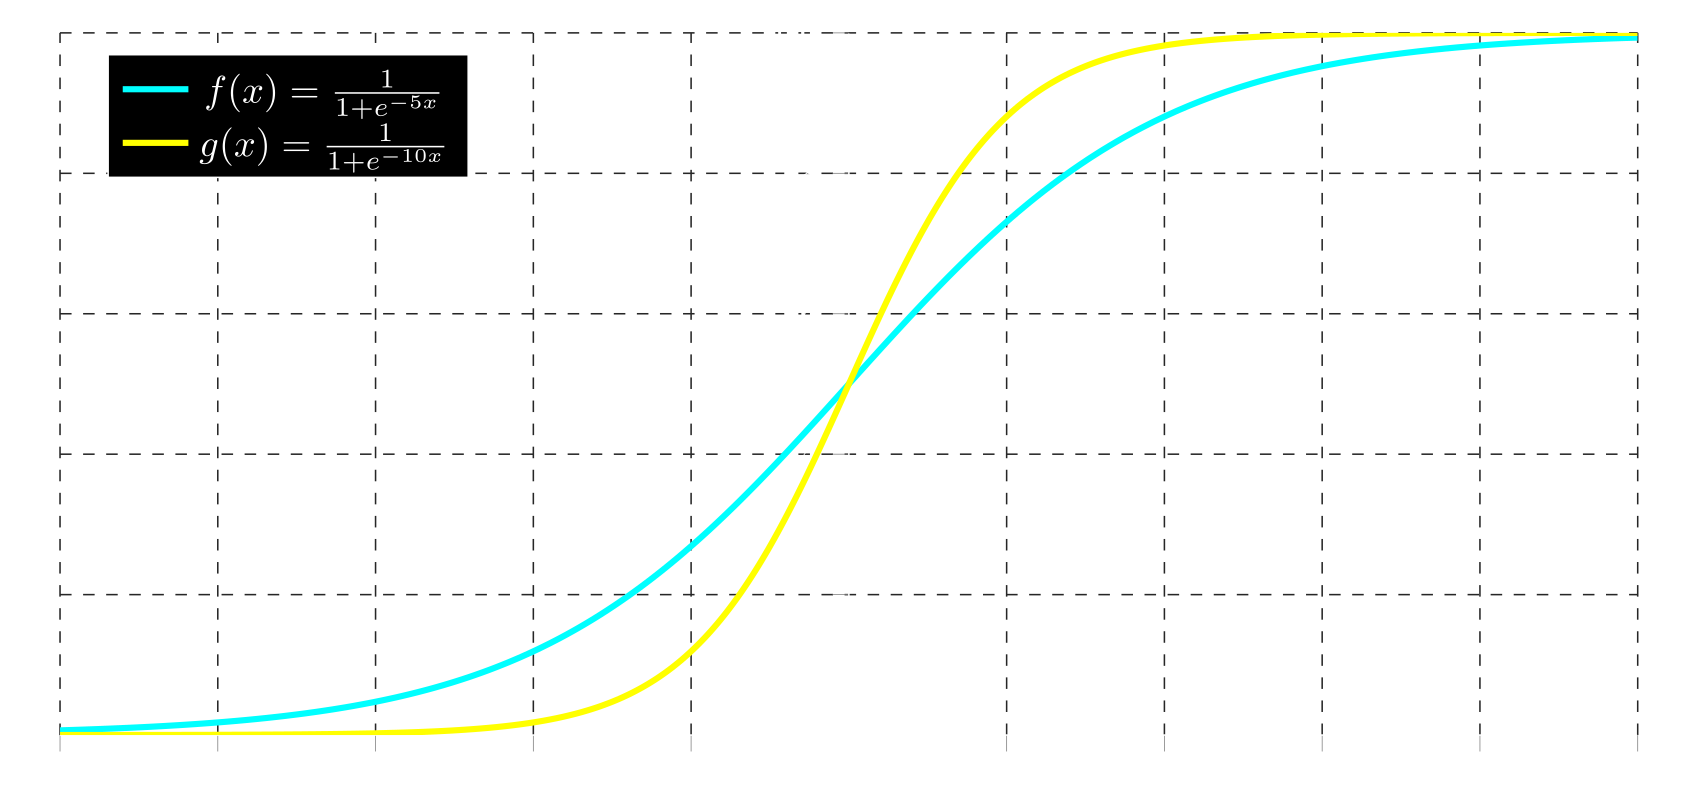
\includegraphics[width=0.4\textwidth]{Sigmoid-function_invertiert.png}
		\tiny\caption{Sigmoide Funktion mit Steigungsmaß
		\textcolor{Turquoise}{a}=5 sowie
		\textcolor{yellow}{a} = 10 \tiny\url{https://de.wikipedia.org/wiki/Datei:Sigmoid-function.svg}}
\end{figure}
\note{alles negativ ist wird bei relu zu 0 während bei sigmoid, abhängig von der Steigung Werte zwischen -1 und 1 möglich sind}
\end{frame}


    
\subsection{Loss/Kostenfunktion}
\begin{frame}[t]{Einleitung zu Neuronalen Netzen}\vspace{4pt}
Loss/Kostenfunktion

\begin{figure}

\center

\textbf{Mean Squared Error}\par\medskip
$MSE=\frac{1}{n}\sum^{n}_{i=1}(Y_i - \hat{Y}_i)^2$

\vspace{2em}
\textbf{Mean absolute error}\par\medskip
$MAE=\frac{\sum^{n}_{i=1}|\hat{y_i}- y_i}{n}$

\vspace{2em}
\textbf{Binary Cross-Entropy}\par\medskip
$H(y, \hat{y})=-\frac{1}{n}\sum^{n}_{i=1} y_i\cdot \log({\hat{y_i}}) + (1-y_i)\cdot\log({1-\hat{y_i}}))$
\vspace{1.5em}
\caption{\tiny\url{https://en.wikipedia.org/wiki/Mean_squared_error\#Predictor}
\tiny\url{https://en.wikipedia.org/wiki/Mean_absolute_error}
{\fontsize{5}{6}\selectfont \url{https://towardsdatascience.com/understanding-binary-cross-entropy-log-loss-a-visual-explanation-a3ac6025181a}}
}
\end{figure}
\note{Man berechnet immer den unterschied zwischen den wahren labeln und den predicteden labeln um zu erkenne wie weit diese auseinander liegen. Es wird immer versucht den Loss zu minimieren. Also ein Minimum der Kostenfunktion zu finden.
Die Parameter der Funktion, welche angepasst werden müssen sind alle weights und biases der einzelnen Neuronen und den Layern.}
\end{frame}

\subsection{Backpropagation mit Gradient descent}
\begin{frame}[t]{Einleitung zu Neuronalen Netzen}\vspace{4pt}
Backpropagation mit Gradient descent

\begin{figure}
    \centering
        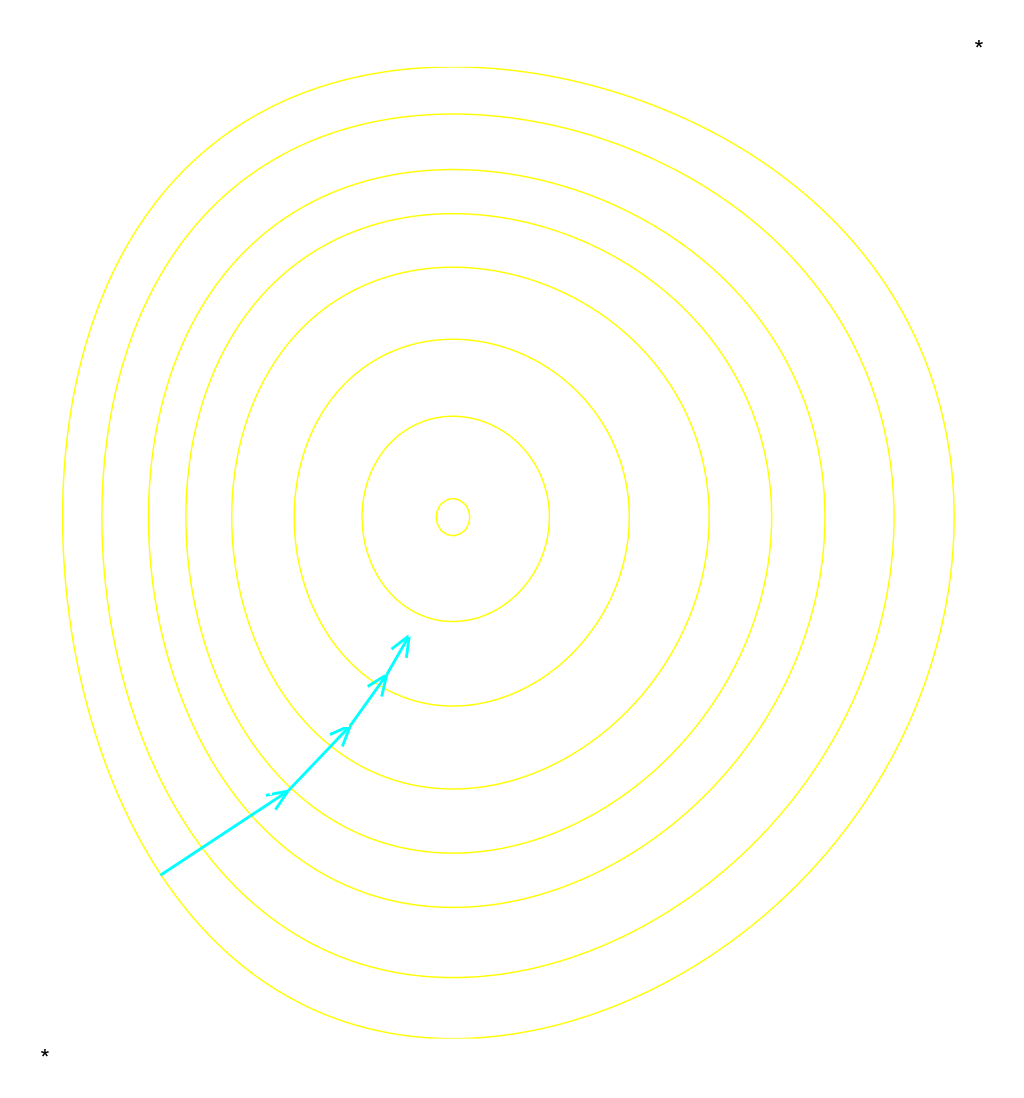
\includegraphics[width=0.5\textwidth]{1024px-Gradient_descent_invertiert.svg.png}
		\tiny\caption{Illustration of gradient descent on a series of \href{https://en.wikipedia.org/wiki/Level_set}{level sets} \tiny\url{https://en.wikipedia.org/wiki/File:Gradient_descent.svg}}
\end{figure}
\note{Über Backpropagation wird hier mit z.B Gradient Descent die Loass funktion minimiert. Der Gradient der Loss/ Kostenfunktion wird für alle wigths and biases gleichzeitig berechnet. Man kann sich das vorstellen, wie eine Kugel die man einen in einer Hügellandschaft rollen lässt ein kleinen schritten und zwischen den schritten immer nach der Steigung des Abhanges schaut und dabei versucht die Kugel in das tiefste Tal zu bekommen. }
\end{frame}

\section{Autoencoders}
\subsection{Idee}
\begin{frame}[t]{Autoencoders}\vspace{4pt}
\begin{center}
\Huge{\begin{itemize}
 \item[] Idee
 \begin{itemize}
 	\LARGE\item[-] Der Input ist der Output
	\LARGE\item[-] Engpass in der Mitte
 \end{itemize}
\note{Ein Autoencoder ist ein feedforward Neural network, was versucht den input zu Kopieren.
Das hört sich im ersten Moment nutzlos an, hat aber doch ein paar Anwendungsmöglichkeiten. Dazu gehört z.B Denosing oder Reduktion des Features Spaces}
\end{itemize}}
\end{center}



\end{frame}

\subsection{Aufbau}
\begin{frame}[t]{Autoencoders}\vspace{4pt}
\begin{figure}
\center
\begin{tikzpicture}
		\node at (0, 0)[](input){Input};
         \node at (2,0) [rectangle,minimum width = 6cm, minimum height = 1cm,rotate=90, draw] (c100) {Encoder};
        \node at (4,0) [rectangle,minimum width = 3cm, minimum height = 1cm,rotate=90, draw] (v100) {Bottleneck};
                 \node at (6,0) [rectangle, minimum width = 6cm, minimum height = 1cm, rotate=90, draw] (v200) {Decoder};
        		\node at (8, 0)[](output){Output};         
        \draw (c100)[-stealth] -- (v100);
        \draw (v100)[-stealth] -- (v200);
        \draw (input)[-stealth] -- (c100);
        \draw (v200)[-stealth] -- (output);
    \end{tikzpicture}
    \caption{Einfaches Autoencoder Model}
\end{figure}
\note{
\begin{itemize}
\item Aufbau, Das Netzwerk besteht im Grunde aus 2 Teilen.
\item Encoder und Decoder
\item Encoder Transformiert die Input Daten in eine kleinere gewünschte Dimension
\item Decoder Transformiert die Daten aus der Kleinen Dimension zurück in die Orginal Dimensionen.
\item Hoffnung das der Encoder die Daten auf die Wichtigsten Features reduziert.
\end{itemize}}
\end{frame}


\begin{frame}[t]{Autoencoders}\vspace{4pt}
\begin{figure}
\center
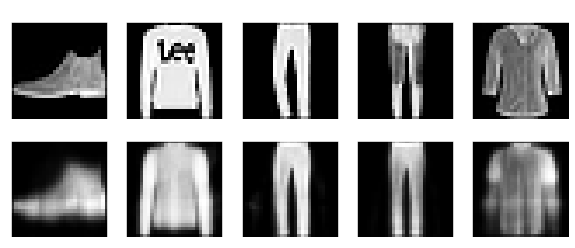
\includegraphics[scale=0.315]{AutoencoderResult.png}
{\fontsize{5}{6}\selectfont \caption{Orginal und Decoded Bilder}}
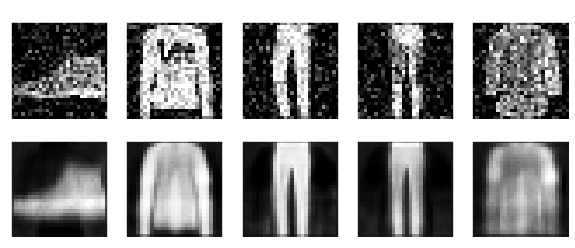
\includegraphics[scale=0.315]{DenosingAutoencoderResult.png}
{\fontsize{5}{6}\selectfont \caption{Noisy und Decoded Bilder}}
\end{figure}
\tiny{\url{https://github.com/Plutokekz/dec/blob/main/Autoencoders.ipynb}}
\note{
\begin{itemize}
\item 784 input zu 10 zu 784 (28*28)
\item Bottleneck size = 10 oder feature redutktion auf 10
\item Random noise 
\end{itemize}
}
\end{frame}

\section[]{Stecked Autoencoders}
	\subsection{Idee}
	\subsection{Aufbau}
\begin{frame}[t]{Stacked Autoencoders}\vspace{4pt}
Idee
Aufbau
\note{
Stacked Autoincoders ist genau das was der name Sagt.\\
mehrere Autoencoder hintereinander.\\
man started mit einem Autoencoder, den man Trainniert.\\
dann entfernt man den decoder Teil\\
und setzt an diese stelle den nächsten Autoencoder, wird wieder trainniert\\
bis die gewünschte anzahl der stacks erreicht ist.\\
Besonderheit man trainiert die folgenden Autoencoder mit dem Output des vorigen encoders.\\
}
\end{frame}

\begin{frame}[t]{Vorherige Arbeiten}\vspace{4pt}
andere Clustering algorithmen ?
andere Dimensions-Reduktions-algorithmen
\end{frame}

\begin{frame}[t]{Von wem ist das Paper}\vspace{4pt}
macvht hier kein sinn kommt am anfang
\end{frame}


\section[]{}
\begin{frame}[t]{Referenzen}\vspace{4pt}
\begin{thebibliography}{10}
\bibitem{Kmeans}
\alert{k-means clustering}
\newblock  {\url{https://en.wikipedia.org/wiki/K-means_clustering\#Complexity}}
\end{thebibliography}

\end{frame}

\end{document}
